 \section{Đề ôn thi giữa kỳ 2 toán 10}
\subsection{Phần trắc nghiệm}
Câu trắc nghiệm nhiều phương án lựa chọn. Học sinh trả lời từ
câu 1 đến câu 12. Mỗi câu hỏi học sinh \textit{chỉ chọn một} phương án.
\Opensolutionfile{ans}[Ans/Dapan] 
\hienthiloigiaiex
%%%=============EX_1=============%%%
\begin{ex} %[0D8H1-2]%[Dự án đề kiểm tra Toán khối 10 GHKII NH23-24-Dot 2-Chu Hà]%[Deso 10 - Sach CD]
	Một học sinh có $4$ quyển sách Toán khác nhau và 5 quyển sách Ngữ văn khác nhau. Hỏi có bao nhiêu cách sắp xếp 9 quyển sách trên giá sách nằm ngang sao cho hai quyển sách kề nhau phải khác loại nhau?
	\choice
	{$362\,880$}
	{\True $2\,880$}
	{$5\,760$}
	{$20$}
	\loigiai{
	Cách sắp xếp phải thỏa mãn theo thứ tự sau: Văn - Toán - Văn - Toán - Văn - Toán - Văn - Toán- Văn.\\
	Vậy có $5 \cdot 4 \cdot 4 \cdot 3 \cdot 3 \cdot 2 \cdot 2 \cdot 1 = 2880$ cách sắp xếp.
		}
\end{ex}
%%%=============EX_2=============%%%
\begin{ex}%[0D8H1-2] %[Dự án đề kiểm tra Toán khối 10 GHKII NH23-24-Dot 2-Chu Hà]%[Deso 10 - Sach CD]
	Có bao nhiêu số tự nhiên có chín chữ số mà các chữ số của nó được viết theo thứ tự giảm dần?
	\choice
	{ $5$}
	{ $15$}
	{ $55$}
	{\True $10$}
	\loigiai{
	Xét theo thứ tự cho sẵn của mười chữ số: $\{9;8;7;6;5;4;3;2;1;0\}$.\\
	Với mõi lần bỏ đi $1$ số từ tập trên và ghép 9 số còn lại thành một số tự nhiên (chú ý giữ nguyên thứ tự ban đầu) thì ta sẽ được một số tự nhiên mới thỏa mãn đề bài.\\
	Vậy có $10$ số tự nhiên thỏa mãn.
	}
\end{ex}
%%%=============EX_3=============%%%
\begin{ex}%[0D8N2-6] %[Dự án đề kiểm tra Toán khối 10 GHKII NH23-24-Dot 2-Chu Hà]%[Deso 10 - Sach CD]
	Cho tứ giác $ABCD$, số vectơ khác $\overrightarrow{0}$ có điểm đầu và điểm cuối là các đỉnh của tứ giác là
	\choice
	{\True $12$}
	{$ 6$}
	{$ 4$}
	{ $10$}
	\loigiai{
		Số vectơ khác  $\overrightarrow{0}$ có điểm đầu và điểm cuối là các đỉnh của tứ giác là $  \mathrm{A}2_4 = 12 $.
	}
\end{ex}
%%%=============EX_4=============%%%
\begin{ex}%[0D8H2-3] %[Dự án đề kiểm tra Toán khối 10 GHKII NH23-24-Dot 2-Chu Hà]%[Deso 10 - Sach CD]
	Cho tập hợp $A=\{1;2;3;4;5;6\}$, từ tập $A$ có thể lập được bao nhiêu số tự nhiên có bốn chữ số khác nhau?
	\choice
	{ $15$}
	{\True $360$}
	{ $24$}
	{ $720$}
	\loigiai{
		Số các số tự nhiên có bốn chữ số khác nhau được lập từ $A$ bằng $\mathrm{A}_6^4 = 360 $ số.
	}
\end{ex}
%%%=============EX_5=============%%%
\begin{ex}%[0D8H2-3] %[Dự án đề kiểm tra Toán khối 10 GHKII NH23-24-Dot 2-Chu Hà]%[Deso 10 - Sach CD]
	Có bao nhiêu số tự nhiên gồm bốn chữ số khác nhau đôi một khác nhau?
	\choice
	{$\mathrm C^4_{10}$}
	{\True $9 \mathrm{A}3_{9}$}
	{$ \mathrm{A}4_{10}$}
	{$9\mathrm C^3_{9}$}
	\loigiai{
	Gọi số tự nhiên có $4$ chữ số khác nhau cần lập là $\overline{abcd}$ với $a\ne 0$. Khi đó:
	\begin{itemize}
	\item Chọn $a$ có $9$ cách chọn.
	\item Chọn $\overline{bcd}$ có $ \mathrm{A}3_9$ cách chọn.
	\end{itemize}
	Vậy có tất cả $9 \mathrm{A}3_{9}$ cách chọn.
	}
\end{ex}
%%%=============EX_6=============%%%
\begin{ex}%[0D8H3-4] %[Dự án đề kiểm tra Toán khối 10 GHKII NH23-24-Dot 2-Chu Hà]%[Deso 10 - Sach CD]
	Trong khai triển nhị thức Newton của $\left( 1+3x\right) ^4$, số hạng thứ $2$ theo số mũ tăng dần của $x$ là?
	\choice
	{$108x$}
	{$54x^2$}
	{$1$}
	{\True $12x$}
	\loigiai{
	Ta có $\left( 1+3x\right)^4=\Sigma^{4}_{k=0}\mathrm C^k_4(3x)^k= \Sigma^{4}_{k=0} \mathrm C^k_4\cdot x^k\cdot 3^k$.\\
	Do đó số hạng thứ $2$ theo số mũ tăng dần của $x$, tương ứng với $k=1$ với $\mathrm C^1_4 (3x)^1$.
	}
\end{ex}
%%%=============EX_7=============%%%
\begin{ex}%[0H9N2-4] %[Dự án đề kiểm tra Toán khối 10 GHKII NH23-24-Dot 2-Chu Hà]%[Deso 10 - Sach CD]
	Cặp vectơ nào dưới đây vuông góc?
	\choice
	{$\overrightarrow{a}=\left(2;-1\right)$ và $\overrightarrow{b}=\left(-3;4 \right)$}
	{$\overrightarrow{a}=\left(3;-4\right)$ và $\overrightarrow{b}=\left(-3;4 \right)$}
	{\True $\overrightarrow{a}=\left(-2;-3\right)$ và $\overrightarrow{b}=\left(6;-4 \right)$}
	{$\overrightarrow{a}=\left(7;-3 \right)$ và $\overrightarrow{b}=\left(3;-7\right)$}
	\loigiai{
	Xét phương án $\overrightarrow{a}=\left(-2;-3 \right)$ và $\overrightarrow{b}=\left(6;-4\right)$, ta có $\overrightarrow{a}\cdot \overrightarrow{b}=-2\cdot 6+3\cdot 4=0\Rightarrow \overrightarrow{a}\perp  \overrightarrow{b}$
	}
\end{ex}
%%%=============EX_8=============%%%
\begin{ex}%[0H9H2-2] %[Dự án đề kiểm tra Toán khối 10 GHKII NH23-24-Dot 2-Chu Hà]%[Deso 10 - Sach CD]
	Trong mặt phẳng $Oxy$, cho $A(1;2), B(4;1), C(5;4)$. Khi đó $\widehat{BAC}$ bằng?
	\choice
	{$60^{\circ}$}
	{\True $45^{\circ}$}
	{$90^{\circ}$}
	{$120^{\circ}$}
	\loigiai{
	Ta có $\overrightarrow{AB}=(3 ;-1)$, $\overrightarrow{AC}=(4;2)$ \[\Rightarrow \cos (\overrightarrow{AB}, \overrightarrow{AC})=\dfrac{\overrightarrow{AB} \cdot \overrightarrow{AC}}{AB \cdot AC}=\dfrac{10}{\sqrt{10} \cdot \sqrt{20}}=\dfrac{\sqrt{2}}{2}.\] 
	$\Rightarrow(\overrightarrow{AB}, \overrightarrow{AC})=45^{\circ}$.
	}
\end{ex}
%%%=============EX_9=============%%%
\begin{ex}%[0H9H4-1] %[Dự án đề kiểm tra Toán khối 10 GHKII NH23-24-Dot 2-Chu Hà]%[Deso 10 - Sach CD]
	Trong mặt phẳng $Oxy$, cho $A\left(4;2\right)$, $B\left(1;-5\right)$. Tìm tâm $I$ đường tròn ngoại tiếp tam giác $OAB$.
	\choice
	{\True $I\left(\dfrac{38}{11}; \dfrac{-21}{11}\right)$}
	{$I\left(\dfrac{5}{3}; 2\right)$}
	{$I\left(\dfrac{38}{11}; \dfrac{21}{11}\right)$}
	{$I\left(\dfrac{1}{3}; \dfrac{7}{3}\right)$}
	\loigiai{
	Gọi $I\left(x;y\right) $ là tâm đường tròn ngoại tiếp tam giác $OAB$.\\
	Ta có $\heva{&O I^2=AI^2\\&OI^2=BI^2} 
	\Leftrightarrow\heva{&x^2+y^2=(x-4)^2+(y-2)^2 \\ &x^2+y^2=\left(x-1\right) ^2+\left( y+5\right)^2}
	\Leftrightarrow\heva{&2x+y=5\\&x-5y=13}
	\Leftrightarrow\heva{&x=\dfrac{38}{11}\\&y=\dfrac{-21}{11}}\\
	\Rightarrow I\left(\dfrac{38}{11}; \dfrac{-21}{11}\right)$.		
	}
\end{ex}
%%%=============EX_10=============%%%
\begin{ex}%[0H9V2-5] %[Dự án đề kiểm tra Toán khối 10 GHKII NH23-24-Dot 2-Chu Hà]%[Deso 10 - Sach CD]
	Trong mặt phẳng $Oxy$. Gọi điểm $B$ là điểm đối xứng với $A$ qua điểm $I\left( -1;2\right) $. Tìm điểm $C$ có hoành độ bằng $-2$ sao cho tam giác $ABC$ vuông tại $C$.
	\choice
	{\True $C\left(-2; 0\right)$ hoặc $C\left(-2; 4\right)$ }
	{$C\left(-2; 1\right)$ hoặc $C\left(-2; 3\right)$ }
	{$C\left(-2; 2\right)$ hoặc $C\left(-2; 2\right)$ }
	{$C\left(-2; -1\right)$ hoặc $C\left(-2; -3\right)$ }
	\loigiai{
	Do $I$ là trung điểm của $AB$ nên $B\left( -3;3 \right) $. Gọi $C\left(-2;t\right)\Rightarrow 
	\heva{&\overrightarrow{CA}=\left(3;1-t\right)\\ &\overrightarrow{CB}=\left(-1;3-t\right)}$.\\
	Tam giác $ABC$ vuông tại $C\Leftrightarrow \overrightarrow{CA}\cdot \overrightarrow{CB}=0 \Leftrightarrow 3 \cdot (-1) + (1-t)(3-t)=0$\\		
	$t^2-4t=0 \Leftrightarrow \hoac{&t=0 \Rightarrow C\left(-2;0\right)\\&t=4 \Rightarrow C\left(-2;4\right)}$.
	}
\end{ex}
%%%=============EX_11=============%%%
\begin{ex}%[0H9V2-5] %[Dự án đề kiểm tra Toán khối 10 GHKII NH23-24-Dot 2-Chu Hà]%[Deso 10 - Sach CD]
	Cho tam giác $ABC$ với $A\left(1;-2\right)$, $B\left(2;-3\right)$, $C\left(3;0\right)$. Tìm giao điểm của đường phân giác ngoài của góc $A$ và đường thẳng $BC$.
	\choice
	{$\left(-1;6\right)$}
	{$\left(1;6\right)$}
	{$\left(-1;-6\right)$}
	{\True $\left(1;-6\right)$}
	\loigiai{
	Ta có $AB=2\sqrt{2}$.
	\begin{center}
	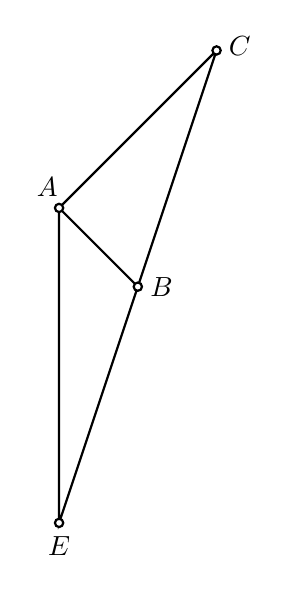
\begin{tikzpicture}[>=stealth,xscale=1,yscale=1,thick]				
	%---Tọa độ điểm - Điểm mới
	\path 
	(1,-2) coordinate (A)	
	(2,-3) coordinate (B)
	(3,0) coordinate (C)
	(1,-6) coordinate (E)
	;
	\draw (C)--(A) --(B)(C)--(E) --(A);
	%---Tên điểm
	\foreach \x/\g in {B/0,A/120,C/10,E/-90}
	\draw[fill=white] (\x) circle (1.5pt)+(\g:0.3)node{$\x$};
	\end{tikzpicture}
	\end{center}		
	Gọi $E$ là chân đường phân giác ngoài tam giác $ABC$ kẻ từ $A$, ta có
	$$\begin{aligned}
	&\dfrac{EC}{EB}=\dfrac{AC}{AB}=2 \Rightarrow \overrightarrow{EC}=2 \overrightarrow{E B} \Rightarrow 
	\heva{3-x_E&=2\left(2-x_E\right) \\	0-y_E&=2\left(-3-y_E\right)}\\
	&\Rightarrow\heva{&x_E=1 \\&y_E=-6}
	\Rightarrow E\left(1;-6\right)
	\end{aligned}$$
	}
\end{ex}
%%%=============EX_12=============%%%
\begin{ex}%[0H9V2-6] %[Dự án đề kiểm tra Toán khối 10 GHKII NH23-24-Dot 2-Chu Hà]%[Deso 10 - Sach CD]
	Cho hai điểm $A\left(-3;1\right)$ và $B\left(-5;5\right)$. Tọa độ điểm $M$ nằm trên trục $Oy$ sao cho $MA-MB$ lớn nhất là
	\choice
	{\True $M\left(0;-5\right)$}
	{$M\left(0;5\right)$}
	{$M\left(0;3\right)$}
	{$M\left(0;-6\right)$}
	\loigiai{
	Nhận thấy $x_A\cdot x_B=15>0$ nên $A$, $B$ cùng phía so với $Oy$.		
	\begin{center}
		\begin{tikzpicture}[>=stealth,xscale=1,yscale=0.65,thick]
		% giá trị phải là số nguyên
		\def\xmax{1}		\def\ymax{6}
		\def\xmin{-6}		\def\ymin{-6}
		%--
		\clip (\xmin.2,\ymin.2) rectangle (\xmax.7,\ymax.7);
		%------Trục tọa độ----
		\draw[->] (\xmin.2,0)--(0,0)node[below left]{$O$} --(\xmax.5,0)node[below]{$x$};
		\draw[->] (0,\ymin.2)--(0,\ymax.5)node[left]{$y$};
		%----Chia trục tọa độ----	
		\foreach \x in {\xmin,...,-1,1,2,...,\xmax}{
		\draw (\x,0.1)--(\x,-0.1) (\x,0) node[below=2pt]{$\x$} ;
			}
		\foreach \x in {-4,-2,2,4}{
		\draw (0.1,\x)--(-0.1,\x) (0,\x) node[left=1.5pt]{$\x$} ;
		}
		\clip (\xmin.3,\ymin.3) rectangle (\xmax.3,\ymax.3);
		%-- Vẽ hàm số ----
		\draw[samples=100,smooth,name path= hs1] 
		plot[domain=\xmin:\xmax] (\x,{-2*(\x)-5})node[below ]{$d$};					
		%---Tọa độ điểm - Điểm mới
		\path (-5,5) coordinate (B)
		(-2.5,0) coordinate (A)	(0,-5) coordinate (M)
		;			
		%---Tên điểm
		\foreach \x/\g in {B/0,A/70,M/10}
		\draw[fill=white] (\x) circle (1.5pt)+(\g:0.3)node{$\x$};
		\end{tikzpicture} 
		\end{center}
	Với $M \in Oy$, ta có $MA-MB\le AB$. Do đó $MA-MB$ lớn nhất bằng $AB$. Khi đó $M,A,B$ thẳng hàng và $M$ nằm ngoài  đoạn $AB$.\\
	Gọi $M(x;y) \Rightarrow \overrightarrow{MA} = (-3;1-y)$ và $\overrightarrow{MB} = (-5;5-y)$.\\
	Vì $\overrightarrow{MA}$ cùng phương với $\overrightarrow{MB}$ nên $\dfrac{-3}{-5}=\dfrac{1-y}{5-y} \Rightarrow y = -5$ hay $M \left( 0;-5\right) $.
	}
\end{ex}
\Closesolutionfile{ans}
\bangdapan{Dapan}

\subsection{Câu trắc nghiệm đúng sai}
Học sinh trả lời từ câu 1 đến câu 4.
Trong mỗi ý \circlenum{A}, \circlenum{B}, \circlenum{C} và \circlenum{D} ở mỗi câu, học sinh chọn đúng hoặc sai.
\setcounter{ex}{0}
\LGexTF
\Opensolutionfile{ansbook}[ansbook/DapanDS]
\Opensolutionfile{ans}[Ans/DapanT]
 %%%============EX_1==============%%%
% \tatloigiaiex
 \begin{ex}%[0D8H2-4]%[Dự án đề kiểm tra Toán khối 10 GHKII NH23-24-Dot 2- Hieu Hieu Minh Minh]%[Deso10 - CD]
 	Một đoàn tàu nhỏ có $3$ toa khách đỗ ở sân ga. Có $3$ hành khách không quen biết cùng bước lên tàu, khi đó:
 	\choiceTF
	{Số khả năng khách lên tàu tùy ý là $9$ khả năng}
	{Số khả năng $3$ hành khách lên cùng một toa là $1$ khả năng}
	{\True Số khả năng mỗi khách lên một toa là $6$ khả năng}
	{\True Số khả năng có $2$ hành khách cùng lên một toa, hành khách thứ ba thì lên toa khác là $18$} 
 	\loigiai{
 	\begin{itemize}
 	\item Khách lên tàu tùy ý nên mỗi khách sẽ có $3$ lựa chọn. Vậy số khả năng thỏa mãn là $3 \times 3 \times 3=27$.
 	\item Số khả năng $3$ hành khách lên cùng một toa là $3$.
 	\item Số cách chọn $3$ toa để xếp $3$ hành khách là $\mathrm{A}_3^3=3!=6$.
 	\item Giai đoạn 1: Chia 3 hành khách ra làm hai nhóm $X$, $Y$: một nhóm có $2$ người và một nhóm có $1$ người. Số cách thực hiện là: $\mathrm{C}_3^2 \times 1$.\\
 	Giai đoạn 2: Chọn $2$ trong $3$ toa tàu để xếp hai nhóm vào, số cách thực hiện là $\mathrm{A}_3^2$.
 	\end{itemize}
 	Vậy số cách xếp khách lên tàu thỏa mãn là $\mathrm{C}_3^2 \times 1 \times \mathrm{A}_3^2=18$.
 	}
 \end{ex}
%%%============EX_2==============%%%
\begin{ex}%[0D8H3-4]%[Dự án đề kiểm tra Toán khối 10 GHKII NH23-24-Dot 2- Hieu Hieu Minh Minh]%[Deso10 - CD]
	Khai triển $(x+2)^5$. Khi đó
	\choiceTF
	{\True Hệ số của $x^4$ trong khai triển là $10$}
	{\True Hệ số của $x^3$ trong khai triển là $40$}
	{Hệ số của $x^2$ trong khai triển là $54$}
	{\True Hệ số của $x$ trong khai triển là $80$} 
	\loigiai{
	\begin{eqnarray*}
	(x+2)^5&=&x^5+5 \cdot x^4 \cdot 2+10 \cdot x^3 \cdot 2^2+10 \cdot x^2 \cdot 2^3+5 \cdot x \cdot 2^4+2^5\\&=&x^5+10 x^4+40 x^3+80 x^2+80 x+32. 
	\end{eqnarray*}
	}
\end{ex}

%%%============EX_3==============%%%
\begin{ex}%[0H9H1-4]%[Dự án đề kiểm tra Toán khối 10 GHKII NH23-24-Dot 2- Hieu Hieu Minh Minh]%[Deso10 - CD]
	Trong mặt phẳng tọa độ $Oxy$, cho các điểm $A\left(-4; 1\right)$, $B\left(2 ; 4\right)$, $C\left(2;-2\right)$.
	\choiceTF
	{Tọa độ điểm $D$ sao cho $C$ là trọng tâm tam giác $ABD$ là $D\left(8 ; 11\right)$}
	{\True Tọa độ điểm $E$ thuộc trục hoành sao cho $A$, $B$, $E$ thẳng hàng là $E\left(-6; 0\right)$}
	{\True $\overrightarrow{BC}=(0 ;-6)$, $\overrightarrow{AC}=\left(6 ;-3\right)$}
	{Tọa độ $F$ thỏa mãn $\overrightarrow{AF}=\overrightarrow{BC}-2 \overrightarrow{AC}+2 \overrightarrow{CF}$ là $F\left(20 ; 5\right)$} 
	\loigiai{
	\begin{itemize}
	\item  $C$ là trọng tâm tam giác $ABD \Leftrightarrow $
	$\heva{&x_C=\dfrac{x_A+x_B+x_D}{3}\\&y_C= \dfrac{y_A+y_B+y_D}{3}\\}
	\Leftrightarrow \heva{&2= \dfrac {-4+2+x_D}{3}\\&-2= \dfrac {1+4+y_D}{3}\\} \Leftrightarrow \heva{&x_D=8\\&y_D=-11.}$ 
	Vậy $D\left(8 ;-11\right)$.
	\item Gọi $E\left(x; 0\right) \in Ox \Rightarrow \overrightarrow{AE}=\left(x+4 ;-1\right), \overrightarrow{AB}=\left(6; 3\right)$.\\
	Ba điểm $A$, $B$, $E$ thẳng hàng $\Leftrightarrow \overrightarrow{AE}$ cùng phương $\overrightarrow{AB}$\\ \begin{eqnarray*}
	&\Leftrightarrow& \dfrac{x+4}{6}=-\dfrac{1}{3}\\ &\Leftrightarrow& x+4=-2\\ &\Leftrightarrow& x=-6.\\
	\end{eqnarray*}
	Vậy $E\left(-6; 0\right)$.
	\item Gọi $F\left(x; y\right)$.\\
	Ta có 
	$\overrightarrow{AF}=\left(x+4; y-1\right)$, $\overrightarrow{BC}=\left(0 ;-6\right)$,\\ $\overrightarrow{AC}=\left(6;-3\right)$
	$\Rightarrow-2 \overrightarrow{AC}=\left(-12; 6\right)$,\\ $\overrightarrow{CF}=\left(x-2; y+2\right)\Rightarrow 2 \overrightarrow{CF}=\left(2x-4; 2y+4\right)$\\
	Suy ra $\overrightarrow{BC}-2 \overrightarrow{AC}+2 \overrightarrow{CF}=\left(2x-16; 2y+4\right)$.\\
	Ta có $ \overrightarrow{AF}=\overrightarrow{BC}-2 \overrightarrow{AC}+2 \overrightarrow{CF} \Leftrightarrow
	\heva{&x+4=2x-16\\&y-1=2y+4} \Leftrightarrow \heva{&x+4=2x=20\\&y=-5.}$\\
	Vậy $F\left(20;-5\right)$.
	\end{itemize}
	}
\end{ex}

%%%============EX_4==============%%%
\begin{ex}%[0H9H3-7]%[Dự án đề kiểm tra Toán khối 10 GHKII NH23-24-Dot 2- Hieu Hieu Minh Minh]%[Deso10 - CD]
	Trong mặt phẳng toạ độ $Oxy$, cho tam giác $ABC$ có $A\left(3;4\right)$, đường trung trực cạnh $BC$ có phương trình $3x-y+1=0$, đường trung tuyến kẻ từ $C$ có phương trình $2x-y+5=0$.
	\choiceTF
	{Gọi $M$ là trung điểm cạnh $BC$. Khi đó $M\left(9;39\right)$}
	{\True Phương trình đường thẳng $B C$ là: $x+3y-63=0$}
	{Tọa độ đỉnh $C$ là $C\left(-1;3\right)$}
	{\True Tọa độ đỉnh $B$ là $B\left(\dfrac{15}{7}; \dfrac{142}{7}\right)$} 
	\loigiai{
	Gọi $M$ là trung điểm cạnh $BC$.\\
	Vì $M$ nằm trên đường trung trực cạnh $BC$ nên giả sử $M(t;3t+1)$.\\
	Gọi $G$ là trọng tâm tam giác $ABC$.\\
	Vì $G$ nằm trên đường trung tuyến kẻ từ $C$ nên giả sử $G(s; 2s+5)$.\\
	Ta có $\overrightarrow{AM}=(t-3;3t-3), \overrightarrow{AG}=(s-3;2s+1)$. Khi đó
	$$\overrightarrow{AM}=\dfrac{3}{2} \overrightarrow{AG}\Leftrightarrow \heva{& t-3=\dfrac{3}{2}\left(s-3\right)\\&3t-3=\dfrac {3}{2}\left(2s+1\right) }
	\Leftrightarrow \heva{&2t-3s=-3\\&6t-6s} \Leftrightarrow \heva{&t=\dfrac{15}{2} \\ &s=6.}$$
	Suy ra $M\left(\dfrac{9}{2}; \dfrac{39}{2}\right)$.\\
	Đường thẳng $BC$ đi qua $M\left(\dfrac{9}{2}; \dfrac{39}{2}\right)$ và vuông góc với đường thẳng $3x-y+1=0$ nên ta có phương trình đường thẳng $BC$ là $1 \cdot\left(x-\dfrac{9}{2}\right)+3 \cdot\left(y-\dfrac{39}{2}\right)=0 \Leftrightarrow x+3y-63=0$.\\
	Tọa độ đỉnh $C$ là nghiệm của hệ phương trình: $\heva{&x+3 y-63=0\\ &2 x-y+5=0} \Leftrightarrow \heva{&x=\dfrac{48}{7}\\ &y=\dfrac{131}{7}.}$\\
	Suy ra $C\left(\dfrac{48}{7} ; \dfrac{131}{7}\right)$.\\
	Vì $M$ là trung điểm $BC$ nên $B\left(\dfrac{15}{7}; \dfrac{142}{7}\right)$.
	}
\end{ex}
\Closesolutionfile{ans}
\Closesolutionfile{ansbook}

\begin{center}
	\textbf{\textsf{BẢNG ĐÁP ÁN ĐÚNG SAI}}
\end{center}
\input{Ansbook/DapanDS}

\subsection{Phần tự luận}
\hienthiloigiaibt
\setcounter{bt}{0}
\begin{bt}%[0D8V3-4]%[Dự án đề kiểm tra toán khối 10 GHKII-NH23-24- Đợt 2-Vanle Vo]%[Deso 10 - Sach CD]%Câu 1.
Gọi $n$ là số nguyên dương thỏa mãn $\mathrm{A}_n^3+2\mathrm{A}_n^2=48$. Tìm hệ số của $x^3$ trong khai triển nhị thức Newton của $(1-3x)^n$.
	\loigiai{
Điều kiện $n \geq 3$, $n \in\mathbb{N}$.
\allowdisplaybreaks
\begin{eqnarray*}
&&\mathrm{A}_n^3+2\mathrm{A}_n^2=48\\
&\Leftrightarrow& \dfrac{n!}{(n-3)!}+2 \cdot \dfrac{n!}{(n-2)!}=48\\
&\Leftrightarrow& n(n-1)(n-2)+2n(n-1)=48\\
&\Leftrightarrow& n^3-n^2-48=0 \Leftrightarrow n=4\text{ (thỏa)}.\\
\end{eqnarray*}
Ta có $(1-3x)^4=\sum\limits_{k=0}^4 \mathrm{C}_4^k(-3x)^k=\sum\limits_{k=0}^4 \mathrm{C}_4^k(-3)^kx^k$.\\
Hệ số của $x^3$ trong khai triển trên ứng với $k=3$.\\
Vậy hệ số của $x^3$ trong khai triển $(1-3x)^4$ là $\mathrm{C}_4^3 \cdot(-3)^3=-108$.
}
\end{bt}

\begin{bt}%[0D8V2-4]%[Dự án đề kiểm tra toán khối 10 GHKII-NH23-24- Đợt 2-Vanle Vo]%[Deso 10 - Sach CD]%Câu 2.
Một đội thanh niên tình nguyện có $15$ người gồm $12$ nam và $3$ nữ. Hỏi có bao nhiêu cách phân công đội thanh niên tình nguyện đó về giúp đỡ $3$ tỉnh miền núi, sao cho mỗi tỉnh có $4$ nam và $1$ nữ?
	\loigiai{
Ta có $\mathrm{C}_3^1\cdot\mathrm{C}_{12}^4$ cách phân công các thanh niên về tỉnh thứ nhất.\\
Với mỗi cách này thì có $\mathrm{C}_2^1 \cdot \mathrm{C}_8^4$ cách phân công số thanh niên còn lại về tỉnh thứ hai.\\
Với mỗi cách phân công trên thì có $\mathrm{C}_1^1\cdot\mathrm{C}_{4}^4$ cách phân công số thanh niên còn lại về tỉnh thứ ba.\\
Do đó, ta có $\mathrm{C}_3^1\cdot\mathrm{C}_{12}^4\cdot\mathrm{C}_2^1\cdot\mathrm{C}_{8}^4\cdot\mathrm{C}_1^1\cdot\mathrm{C}_{4}^4=207900$ cách phân công thỏa mãn đề bài.\\
Gọi số cần lập có dạng $abc$.\\
Chọn $c$ với $c \in\{4;6;8\}$ có $3$ cách.\\
Chọn $\overline{ab}$ có $\mathrm{A}_5^2$ cách.\\
Theo quy tắc nhân, ta có $3 \cdot \mathrm{A}_5^2=60$ số tự nhiên thỏa mãn.
}
\end{bt}

\begin{bt}%[0D8V2-6]%[Dự án đề kiểm tra toán khối 10 GHKII-NH23-24- Đợt 2-Vanle Vo]%[Deso 10 - Sach CD]%Câu 3.
Một đa giác đều có $44$ đường chéo, hỏi số cạnh của đa giác đó bằng bao nhiêu?
	\loigiai{
Hai đỉnh của đa giác $n$ đỉnh ($n \in \mathbb{N}$, $n \geq 3$) tạo thành một đọan thẳng (bao gồm cả cạnh và đường chéo của đa giác đó).\\
Vậy số đường chéo đa giác là
\allowdisplaybreaks
\begin{eqnarray*}
&&\mathrm{C}_n^2-n=44 \Leftrightarrow \dfrac{n !}{(n-2)!\cdot 2!}-n=44\\
&\Leftrightarrow& n(n-1)-2 n=88 \Leftrightarrow\hoac{&n=11\\&n=-8}
\Leftrightarrow n=11\text { (vì } n \in \mathbb{N}).
\end{eqnarray*}
}
\end{bt}

\begin{bt}%[0H9V1-4]%[Dự án đề kiểm tra toán khối 10 GHKII-NH23-24- Đợt 2-Vanle Vo]%[Deso 10 - Sach CD]%Câu 4.
Trong mặt phẳng tọa độ $Oxy$, cho ba điểm $A(-1;4)$, $B(1;1)$, $C(3;-1)$. Tìm điểm $N$ thuộc trục hoành sao cho $|NA-NC|$ bé nhất.
	\loigiai{
Ta thấy $y_A \cdot y_C=4 \cdot(-1)<0$ nên $A$, $C$ nằm khác phía so với trục $Ox$.\\
Lấy điểm $C'$ đối xứng với $C$ qua $Ox$. Suy ra $C'(3;1)$ và $C'$, $A$ cùng phía so với $Ox$.\\
Ta có $N \in Ox \Rightarrow NC=NC'$. Vì vậy $|NA-NC|=\left|NA-NC'\right|\leq A C'$.\\
Suy ra $|NA-NC|_{\max}=AC'$; giá trị lớn nhất này đạt được khi $A$, $C$, $N$ thẳng hàng ($N$ nằm ngoài $A$, $C'$).\\
Gọi $N(a;0) \in Ox \Rightarrow \overrightarrow{AN}=(a+1;-4), \overrightarrow{AC'}=(4;-3)$.\\
Vì $\overrightarrow{AN}, \overrightarrow{AC'}$ cùng phương nên $\dfrac{a+1}{4}=\dfrac{-4}{-3} \Leftrightarrow-3a-3=-16 \Leftrightarrow a=\dfrac{13}{3}$.\\
Vậy $N\left(\dfrac{13}{3};0\right)$ thỏa mãn đề bài.
}
\end{bt}

\begin{bt}%[0H9V3-6]%[Dự án đề kiểm tra toán khối 10 GHKII-NH23-24- Đợt 2-Vanle Vo]%[Deso 10 - Sach CD]%Câu 5.
Trong mặt phẳng tọa độ $Oxy$, cho $A(1;6)$, $B(-3;4)$, $\Delta\colon\heva{&x=1+t\\&y=1+2t}(t \in \mathbb{R})$. Tìm $N \in \Delta$ sao cho khoảng cách từ gốc tọa độ $O$ đến $N$ nhỏ nhất.
	\loigiai{
$N \in \Delta$ để $ON$ nhỏ nhất thì $ON \perp \Delta$.\\
$N\in \Delta \Rightarrow N(1+t;1+2t),t\in\mathbb{R}$; $\overrightarrow{ON}=(1+t;1+2t)$.\\
Vectơ chỉ phương của $\Delta$ là $\overrightarrow{u}_{\Delta}=(1;2)$.\\
Vì $ON \perp \Delta \Rightarrow \overrightarrow{ON} \perp \overrightarrow{u}_{\Delta}\Leftrightarrow \overrightarrow{ON} \cdot \overrightarrow{u}_{\Delta}=0 \Leftrightarrow 1(1+t)+2(1+2t)=0 \Leftrightarrow t=\dfrac{-3}{5} \Rightarrow N\left(\dfrac{2}{5}; \dfrac{-1}{5}\right)$.
}
\end{bt}

\begin{bt}%[0H9V1-3]%[Dự án đề kiểm tra toán khối 10 GHKII-NH23-24- Đợt 2-Vanle Vo]%[Deso 10 - Sach CD]%Câu 6.
Trong mặt phẳng tọa độ $Oxy$, cho điểm $A(2;4)$ và đường thẳng $d\colon x+7y-5=0$. Tìm tọa độ điểm $M$ có tung độ dương thuộc đường thẳng $d$ sao cho $A M=5$.
	\loigiai{
Điểm $M$ thuộc đường thẳng $d\colon x+7y-5=0 \Rightarrow M(-7a+5;a)$ ($a>0$).\\
$\overrightarrow{AM}=(-7a+3;a-4)\Rightarrow AM=5\Leftrightarrow (-7a+3)^2+(a-4)^2=25$.\\
Vậy $a=1 \Rightarrow M(-2;1)$. 
}
\end{bt} 

